% Use class option [extendedabs] to prepare the 1-page extended abstract.
\documentclass[extendedabs]{bmvc2k}
\usepackage[colorlinks = true,
            linkcolor = blue,
            urlcolor  = blue,
            citecolor = blue,
            anchorcolor = blue]{hyperref}
\usepackage{kotex} % 한국어 사용 가능

% Document starts here
\begin{document}
\title{eXplainable Artificial Intelligence(XAI)}
\addauthor{
Lee Gwan Hui$^1$, \today}{}{1}
\addinstitution{
$^1$2017142136, Department of Electrical and Electronic Engineering, Yonsei University.}
\maketitle
\let\thefootnote\relax\footnote{This is an extended abstract. The full paper is available at the \href{https://github.com/LeeGwanHui/TIL/tree/main/deeplearning_ham}{github}. }
\vspace{-0.2in}

\section{(XAI(Explainable AI)란\cite{youtubeXAI}}
 \quad XAI란 인공지능 model를 개발하고 그 model을 분석하는 tool이다.\cite{h} XAI는 인공지능 model이 Black Box problem이 있다는 것에서 출발한다.
 Black Box problem이란 input을 model에 통과시켜 얻는 output을 살펴볼 때 왜 원하는 해답을 내놓는지 혹은 원치않는 답을 내놓는지를 파악할 수 없다는 것이다.
 XAI는 특히 의료분야나 자율주행 분야 등 정밀한 분석이 필요한 시스템에 필수적인 요소이며 error의 발생 원인을 detect하고 고칠 수 있도록 insight를 준다.
 XAI 방법은 대표적으로 Backward-based methods 가 있다. Backward-based methods의 초창기 방법으로는 Saliency Map이 있는데 여기서는 좀 더 발전된 형태인
 CAM(Class Activation Map)과 Grad-CAM(Gradient-based Class Activation Map)을 살펴볼 것이다.

\section{CAM(Class Activation Map)\cite{zhou2016learning}}

 \subsection{motivation}
 \quad CNN layer의 convolutional unit은 object detector의 역할을 하기도 하지만 FC layer를 통과하면서 localization정보를 잃는다.
 그래서 parameter수를 줄이는 것과 동시에 localization 정보를 유지하기 위해서 GAP(global average pooling)을 사용하여 remarkable localization ability을 가지는
 model을 제안할 것이다. 이를 통해 classification task로 학습된 model로 더 고차원의 task인 object detection같은 task에 사용될 수 있도록 activation map을 뽑아볼 것이다.

 \subsection{Related work}
 \quad Weakly-supervised object localization이란 label을 이용하여 localization을 하는 것이다. 가장 먼저 해야 할 일은 FC layer을 제거하는 일이다. FC layer은 
 layer의 정보가 어떻게 backpropagation 되는지 알기가 어렵고 parameter수도 많다는 단점이 있다. 그래서 결론적으로 localization 정보를 추출하기에 매우 번거롭다. 그래서
 기존의 논문의 경우에는 GMP(global Max pooling)을 사용했는데 이는 최댓값만 뽑아내는 거다보니 localization 정보를 잃게 된다. 그래서 이 논문에서는 GAP를 사용하여 
 어떤 feature map이 높은 confidence를 갖는지 확인을 용이하게 하고 전 과정에 대해 activation map을 출력할 수 있도록 설계하였다.
 
\subsection{CAM의 구조}
 \quad softmax layer 전에 GAP를 수행하고 이를 FC layer에 대한 feature로써 사용할 것이다. 전체적인 구조는 아래와 같다. 
 \newline  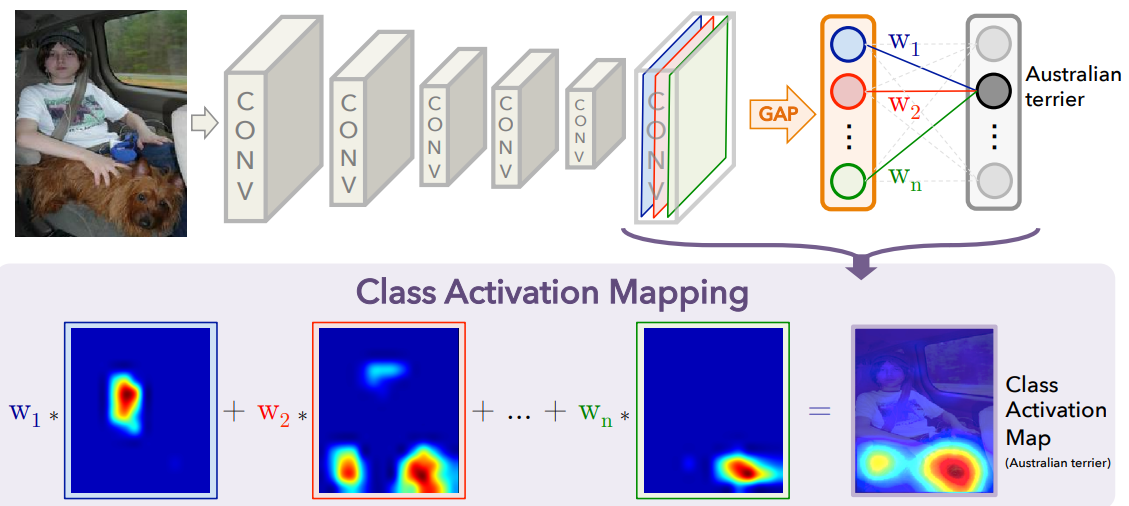
\includegraphics[width=\linewidth]{images/00_CAM.PNG}
 식으로 간단히 표현하자면 $f_k(x,y)$ 는 k번째 feature map에 x,y를 의미한다. GAP를 적용한 결과는 $F^k= \Sigma_{x,y}f_k(x,y)$ 로 나타내자. 전체로 나누는 과정은 편의상 생략했다.
 class c에 대한 softmax의 input은 $S_c=\Sigma_k w_c^cF_k$ 라고 나타낸다. 결론적으로 $w_c^k$ 는 class c에 대한 $F_k$ 의 importance를 나타낸다.
 마지막으로 class c에 대한 softmax의 output은 $P_c=\frac{exp(S_C)}{\Sigma_c exp(S_C)}$ 로 나타낸다.
 즉 $S_c=\Sigma_k w_c^cF_k = \Sigma_k w_c^c \Sigma_{x,y}f_k(x,y) = \Sigma_{x,y} \Sigma_k w_k^c f_k(x,y) = \Sigma_{x,y}M_c(x,y)$ 로 쓸 수 있다.
 여기서 $M_c(x,y)$ 는 class c에 대한 (x,y)에서 class activation map을 나타낸다. 이 값을 간단히 input size로 upsampling하면 아래 처럼 classification을 위해 어디를 중심으로 봤는지 확인할 수 있다.
 \newline  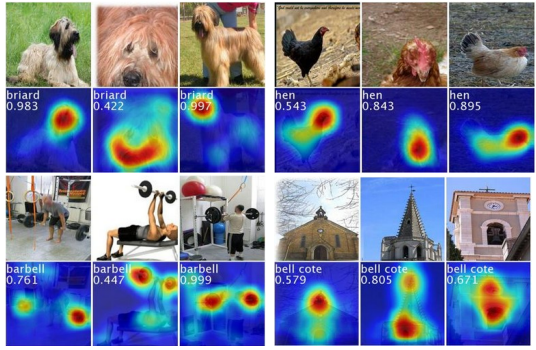
\includegraphics[width=\linewidth]{images/01_CAM.PNG}

 \subsection{실험}
 \quad 이 논문은 AlexNet, VGGnet, GooLeNet, NIN 과 비교를 했다. CAM의 구조를 삽입하기 위해서 FC layer를 제거하는 과정에서 model의 수정이 들어갔다. 실험은
  크게 Classification과 localization으로 나뉘어서 각 error을 비교하였다. 그 결과 classification에서는 아래와 같은 기존 모델과 크게 차이 나지 않는 결과를 얻을 수 있었다.  
  \newline  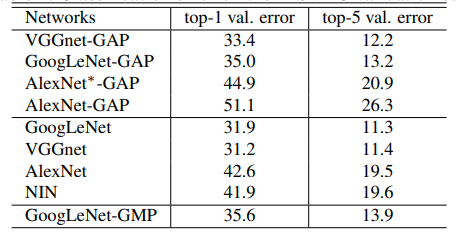
\includegraphics[width=5cm]{images/02_CAM.PNG}
  \newline localization의 경우 bounding box를 생성해주는 algorithm이 필요하다. 이 논문에서는 thresholding 기술을 사용하였다. 
  첫번째로 CAM의 max 값에 해당하는 20\% 값 위의 값을 segment한 후 아래와 같이\cite{youtubeCAM} segmentation map안에 largest connected component를 cover하는 bounding box를 잡는다. 
  \newline  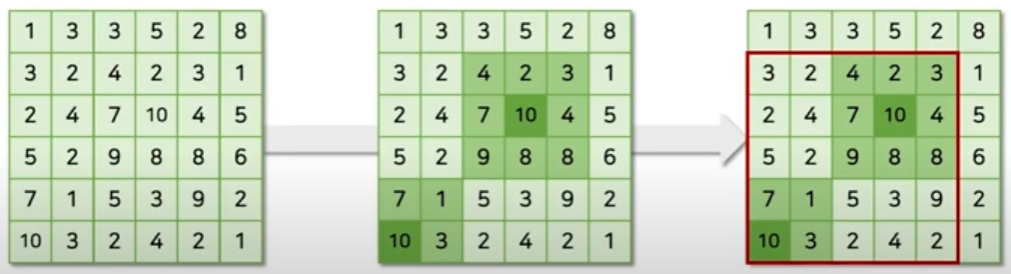
\includegraphics[width=\linewidth]{images/03_CAM.PNG}
  그 결과 localization의 경우에는 GoogLeNet-GAP의 경우 top-1 val.error가 56.40, top-5 val.error가 43.00 으로 가장 좋은 결과를 얻을 수 있었다. 이는 GMP를 사용한 결과보다 더 좋았기 때문에
  GAP가 GMP보다 공간적인 정보를 잘 포함한다는 이 논문의 예상과 일치한다. 물론 bounding box가 있는 경우보다는 error가 높지만 그래도 classification결과로 localization task를 일부해결할 수 있다는 것에 의의가 있다.
  그리고 classification task를 진행할 때 어떤 영역을 보고 object label을 결정하는지 파악할 수 있다.
  
  \subsection{Conclusion}
  \quad 이 논문에서는 GAP를 사용한 CNN을 위한 CAM 기술을 제안하였고 그 결과 classification task로 학습시킨 모델이 localization에서도 이용할 수 있다는 것을 확인할 수 있었다.
  사실 이것보다도 Class activation map은 예상한 class score가 나오기 까지 어떤 부분을 중심으로 봤는지 확인할 수 있도록 visualize 할 수 있어 XAI 분야의 발전에 큰 영향을 미쳤다.

\section{Grad-CAM(Gradient-based Class Activation Map)\cite{selvaraju2017grad}}
 \subsection{motivation}
 \quad Grad-CAM역시 XAI 분야에서 모델의 성능 평가를 시각화하는 것인데 CAM의 한계인 GAP의 구조를 가지도록 기존의 CNN의 구조를 수정해야 한다는 점을
 보완한 논문이다. 즉, Grad-CAM의 가장 큰 장점은 어떤 CNN model에도 적용할 수 있다는 것이다. 
 
 \subsection{Related work\cite{youtubeGradCAM}}
 \quad 기존의 논문의 경우에 Accuracy와 simplicity or interpretablility는 trade off 관계가 있었다.
 하지만 이 논문에서는 이러한 trade-off 관계를 깨버린 아이디어를 제시한다. 또한 좋은 visual explanation이란 class discriminative 즉 한 이미지에서 class를 구별할 수 있어야 하고 충분히 object를 판별할 수 있고
 특징을 알아낼 수 있도록 high-resolution을 가져야 한다.기존의 Guided Backpropagation and Deconvolution의 경우에는 high-resolution하지만 class-discriminative가 아쉬웠다. 
 반면 Grad-CAM은 class discriminative에 장점이 있다. 그래서 두가지 특징을 결합한 Guided Grad CAM을 만들기도 한다.
 
 \subsection{Grad-CAM의 구조와 설명}
 \quad Grad-CAM의 핵심 아이디어는 CAM의 GAP를 대신할 수 있도록 feature의 특징을 가지고 있는 값을 뽑아내는 것이다. 우리는 이전 연구들을 통해서 layer가 깊어질수록 specific한 구조적 정보를 얻을 수 있다는 것을 안다. 
 따라서 마지막 CNN layer에서 가장 high-level semantic 정보와 spatial information을 가지고 있을 것이고 이를 이용하기 위해서 마지막 layer에 흘러들어가는 gradient를 이용해서 모델 예측에 
 각 neuron이 미치는 영향을 파악하는게 핵심이다. Grad-CAM 구조는 아래와 같다. 
 \newline  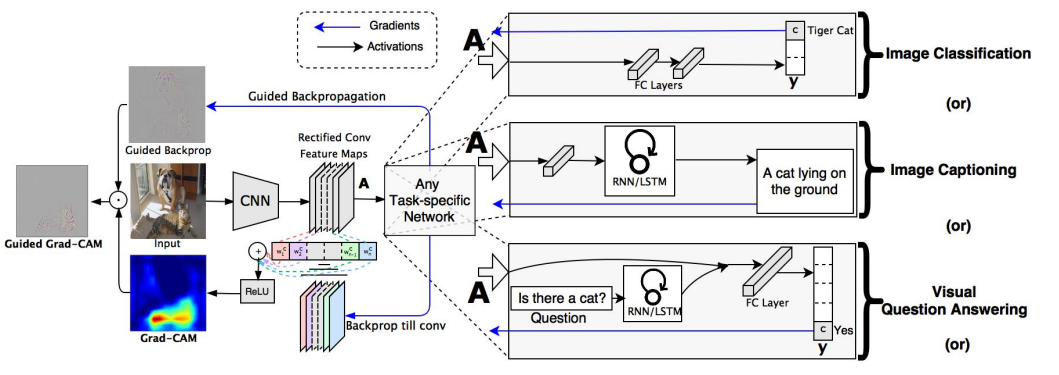
\includegraphics[width=\linewidth]{images/04_CAM.PNG}
 grad-CAM의 수식적 표현을 정의하기 위해 class-discriminative localization map Grad-CAM $L^c_{Grad-CAM} \in R^{ u \times v}$ 을 정의하자 여기서 u와 v는 각각 width와 height이다.
 우리는 class c의 score $y^c$의 gradient 를 구해야 한다. 즉, $\frac{\delta y_c}{\delta A^k}$을 구해야 한다. 이렇게 식을 새우면 neuron importance weights $\alpha^c_k$ 는 
 각 pixel 의 크기로 모두 더해주어야 하므로 아래와 같이 쓸 수 있다. 
 \newline  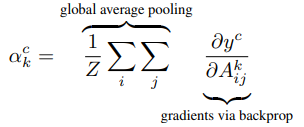
\includegraphics[width=3cm]{images/05_CAM.PNG}
 \newline 그리고 $L^c_{Grad-CAM}$ 의 경우에는 이 값이 양인 값만 볼 거기 때문에 (음의 값은 다른 class를 나타낼 확률이 높다.) ReLU function을 통과시켜주면 아래와 같다.
 \newline  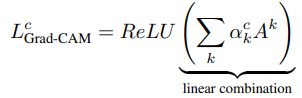
\includegraphics[width=3cm]{images/06_CAM.PNG}
 \newline 이제 할 것은 CAM의 GAP를 진짜 gradient로 대체 가능한지 증명하는 일이다. 이 증명은 Grad-CAM이 CAM의 일반화 형태라는 것으로 증명한다.
 \newline  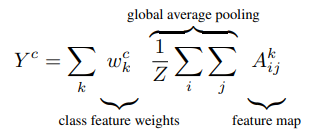
\includegraphics[width=3cm]{images/07_CAM.PNG}
 \newline 위 식은 CAM에 관한 식이다. 여기서 $F^k = \frac{1}{Z}\Sigma_i\Sigma_j A^k_{ij}$라고 정의하면 $Y^c = \Sigma_k w_k^c F^k $ 로 나타낼 수 있다.
 한편 $\frac{\delta Y_c}{\delta F^k}=\frac{\frac{\delta Y^c}{\delta A^k_{ij}}}{\frac{\delta F^k}{\delta A^k_{ij}}}$ 라고 쓸 수 있고 $F^k$의 정의에 따라 $\frac{∂F^k}{\delta A^k_{ij}}=\frac{1}{Z}$ 이다.
 따라서 $\frac{\delta Y_c}{\delta F^k}=\frac{\delta Y^c}{\delta A^k_{ij}}Z$이고 여기에 $Y^c$의 정의를 이용해서 $F^k$를 편미분한 값을 나타내면 $w_k^c=Z\frac{\delta Y^c}{\delta A^k_{ij}}$ 값을 얻을 수 있다.
 마지막으로 이 값을 모든 i와 j에 대해서 더하게 되면 $w_k^c=\Sigma_i \Sigma_j \frac{\delta Y^c}{\delta A^k_{ij}}$을 얻을 수 있다.
 이것을 Grad-CAM의 $\alpha_k^c$와 비교해보면 1/Z 빼고 식이 같다. 즉 CNN의 마지막에 GAP를 사용하는 것이 CAM인데 이때는 Grad-CAM의 특별한 경우로 볼 수 있다는 것이다.
 따라서 Grad-CAM은 CAM을 일반화한 버전이다.
 앞서 첨부한 그림에서 전체적인 구조를 살펴보면 Grad-CAM이랑 Guided Backprop을 element-wise 곱을 통해서 Guided-Grad-CAM을 만든것을 볼 수 있을 것이다. 이 구조의 특징은 위에 Related work에서 언급했듯이 
 high-resolution과 class-discriminative을 만족한다. 
 
 \subsection{실험}
 \quad localization performance를 먼저 살펴보자면 VGG-16을 사용했을 때 model의 변형이 없기 때문에 classification error는 기존 모델과 같고 localization의 결과는 Top-1를 봤을 때
 CAM에 비해 성능이 더 좋았다. 사람의 직접 평가도 추가했는데 그 기준은 Which of the two object categories is depicted in the image?로 묻는 것이었다.
 그 결과 Guide Grad-CAM의 경우 Human Accuracy가 61.23\% 가 나와서  Guided Backpropagation보다 더 좋은 결과를 냈다. XAI를 연구하는 가장 큰 이유는 잘못 판단 내릴 때 무엇 때문에 잘못 판단했는지 결론을 내리기 위해서이다.
 그래서 이 논문에서는 VGG-16 model이 잘못 판단 내린 결과를 visualize하여 모델을 분석한다. 
 \newline  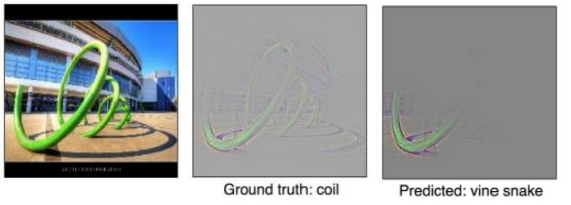
\includegraphics[width=\linewidth]{images/08_CAM.PNG}
 위의 결과를 설명하자면 coil이라고 예상해야 하는 것을 snake로 예상한 것이다. snake로 판단하는 이유를 생각해볼때 coil의 일부분만을 보고 snake로 판단했음을 알 수 있다. 
 아래의 결과는 78\%의 의사가 남자이고 93\%의 간호사가 여성인 편향된 data를 학습시켰을 때의 결과이다. 이 결과를 보면 머리가 길고 여성이라는 것을 보고 nurse라고 판단하고 의사 사진 input의 경우에도 
 성별만 보고 nurse라고 판단한 것을 확인할 수 있었다. 이를 고치기 위해서 unbiased된 data로 학습시켜주면 청진기 혹은 옷의 길이 같은 성별의 특징이 아닌 것으로 직업을 판단하였다.
 \newline  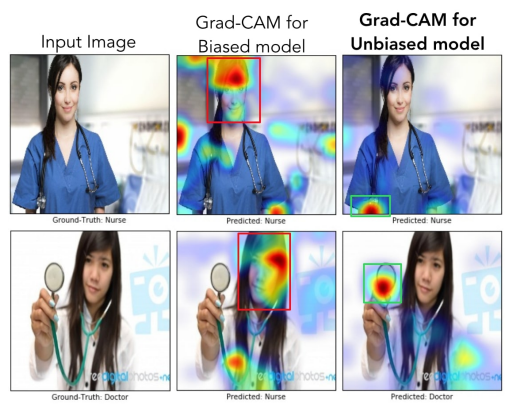
\includegraphics[width=8cm]{images/09_CAM.PNG}
 \newline  위와 같은 오류가 있는 model을 수정할 때 보다 전체적인 구조를 살펴보도록 algorithm을 바꾸거나 coil에 해당하는 것을 추가로 학습시키는 방법을 사용할 수 있을 것이다. 이처럼 XAI는 딥러닝 model을 분석하는 하나의 tool의 개념으로 더 높은 성능을 위해 혹은 더 정밀한 실사용을 위해
 주목받는 분야이다.

 \subsection{Conclusion}
 \quad 마지막 CNN layer의 gradient를 이용한 Grad-CAM을 통해 CAM의 구조적인 한계를 극복하였다. 그리고 기존의 고해상도 시각화 기술을 결합하여 Guided Grad-CAM을 만들었다. 이로 인해 인간 연구를 진행한 결과
 기존 연구보다 더 확실하게 classification결과든지 localization결과 등 의미 있는 결과를 보임을 입증했다. 

\newpage
\bibliography{egbib}

\end{document}